\documentclass[xcolor=svgnames,ngerman]{beamer}
\usetheme{DarkHU}

%\usepackage{pgfpages}
%\pgfpagesuselayout{2 on 1}[a4paper,border shrink=5mm]

\usepackage[utf8]{inputenc}
\usepackage[T1]{fontenc}
\usepackage{lmodern}
\usepackage[ngerman]{babel}

\usepackage{amsmath}
%\usepackage{amsfonts}
\usepackage{amssymb}
\usepackage{mathtools}

\usepackage{eurosym}

%\usepackage[backend=biber, style=authortitle-icomp]{biblatex}
\usepackage[babel,german=guillemets]{csquotes}
%\addbibresource{bib.bib}

%\usepackage{algorithm}
%\usepackage{algpseudocode}

\usepackage{tikz}
\usetikzlibrary{shapes, fit, positioning}
\usepackage{hyperref}

%%%%%%%%%%%%%%%%%%%%%%%
% UTF-8 input encoding
\usepackage[utf8]{inputenc}
\usepackage{microtype}\usepackage{blindtext}

% Page layout formating of koma-script
\usepackage[automark]{scrpage2}
\usepackage{lmodern}

% Language support
\usepackage[ngerman]{babel}

% AMSMath package
\usepackage{amsfonts}
\usepackage{amssymb}
\usepackage{amstext}
\usepackage{amsopn}
\usepackage{amsthm}
\usepackage{url}
\usepackage{listings}
\usepackage{xspace}
\usepackage{mathabx}
%\usepackage{mathptmx}
\usepackage{esint}
\usepackage{graphicx}
\usepackage{mathtools}
\usepackage{hyperref}

%%%%%%%%%%%%%%%%%%%%%%%%%
\usepackage{enumitem,amssymb}
\newlist{todolist}{itemize}{2}
\setlist[todolist]{label=$\square$}
\usepackage{pifont}
\newcommand{\cmark}{\ding{51}}%
\newcommand{\xmark}{\ding{55}}%
\newcommand{\done}{\rlap{$\square$}{\raisebox{2pt}{\large\hspace{1pt}\cmark}}%
\hspace{-2.5pt}}
\newcommand{\wontfix}{\rlap{$\square$}{\large\hspace{1pt}\xmark}}
%%%%%%%%%%%%%%%%%%%%%%%%%%%


\parindent 0ex


\providecommand{\integral}[3]{\ensuremath{\int\limits_{#1} \! {#2} \, \mathrm{d}#3}}
\providecommand{\T}{\ensuremath{\mathcal{T}}}
\providecommand{\Hh}{\ensuremath{\mathrm{H}}}
\providecommand{\Ll}{\ensuremath{\mathrm{L}}}
 
%%%%%%%%%%
\setbeamercolor{green box}{use=base, fg=base.fg, bg=green}
\newenvironment{question}[1][center]{\begin{beamercolorbox}[#1, rounded=true, sep=1pt]{green box}}{\end{beamercolorbox}}

\setbeamercolor{yellow box}{use=base, fg=base.fg, bg=yellow}
\newenvironment{emphbox}[1][center]{\begin{beamercolorbox}[#1, rounded=true, sep=1pt]{yellow box}}{\end{beamercolorbox}}

\renewcommand{\emph}[1]{\textcolor{magenta}{\bfseries #1}}
\providecommand{\abs}[1]{\ensuremath{\left\lvert#1\right\rvert}}

%\setbeamercovered{transparent}
%\setbeamertemplate{navigation symbols}{}

%%%%%%%%%%%%%%%%%%%%%%%%%%%%%%%%%%%%%%%%%%%%%%%%%%%%%%%%%%%%
\author{Enrico Bergmann, Leonard Richter-Matthies, Maximilian Schade}
\title{Verschiedene Polynomgrade im Ansatz- und Testraum}
\subtitle{Zwischenpräsentation}
\institute{Humboldt-Universität zu Berlin}
\date{\today}
\titlegraphic{
\includegraphics[height=1.6cm]{hukombi_bbw_rgb_op}}
%%%%%%%%%%%%%%%%%%%%%%%%%%%%%%%%%%%%%%%%%%%%%%%%%%%%%%%%%%%%

\usepackage{microtype}
\begin{document}
	\maketitle
	\begin{frame}
Wir suchen $(u,t)\in \Hh_0^1(\Omega) \times \Hh^{-1/2}(\partial \T) \eqqcolon X$, sodass
$$b((u,t),v)\coloneqq\integral{\Omega}{\nabla u\cdot\nabla_{NC}v}{x}-\sum\limits_{T\in\T}\integral{\partial T} {v\ t_T}{s}=\integral{\Omega}{f\, v}{x}\eqqcolon F(v)$$
für alle $v\in \Hh^1(\T)\eqqcolon Y$ erfüllt ist.\\ Dafür betrachten wir für die Diskretisierung die Unterräume $S^{k_u}(\T)\subset \Hh^1(\T)$, $P_{k_q}(\mathcal{E})\subset \Hh^{-1/2}(\partial\T)$ und $P_{k_v}(\T)\subset \Hh^1(\T)$ auf einer regulären Triangulierung $\T$ von $\Omega$ in abgeschlossene Dreiecke. Speziell werden wir dafür die drei Fälle
\begin{center}
\begin{tabular}{l | l l l}
	& $k_u$ & $k_q$ & $k_v$\\\hline
	Fall 1 & $k$ & $k-1$ & $k+1$ \\
	Fall 2 & $k-1$ & $k-1$ & $k$ \\
	Fall 3 & $k$ & $k-1$ & $k$ 
\end{tabular}
\end{center}
für $k_u,k_q,k_v=1,2,3$ betrachten. 


\end{frame}

\begin{frame}{Checkliste}
\begin{itemize}
  \item
  \begin{todolist}
  \item[\done] $P_1$ implementieren.
  \item[\done] $P_2$ implementieren.
\pause  
  \item $P_3$ implementieren.
  \item Implementation des eingebauten Fehlerschätzers.
  \item Nachstellen der Experimente aus dem Paper.
  \pause
  \item[\wontfix] Optimierung des Codes.
  \item[\wontfix] Durchführung weiterer Experimente.
  \item[\wontfix] Auswertung und Dokumentation.
  
  \end{todolist}
\end{itemize}
\end{frame}	
	
	\begin{frame}{Approximation von $u$ für $-\Delta u =1$, $u_{|\partial \Omega}=0  $ }
	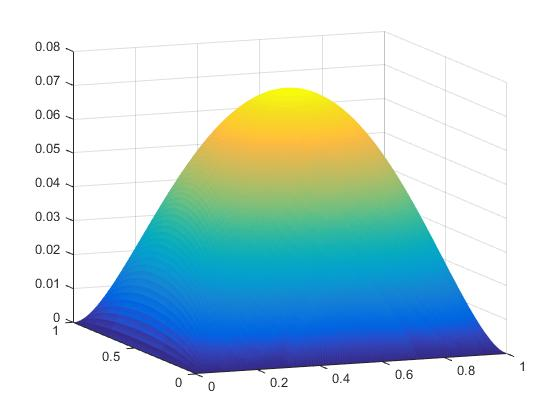
\includegraphics[scale=0.3]{solution1.jpg}
	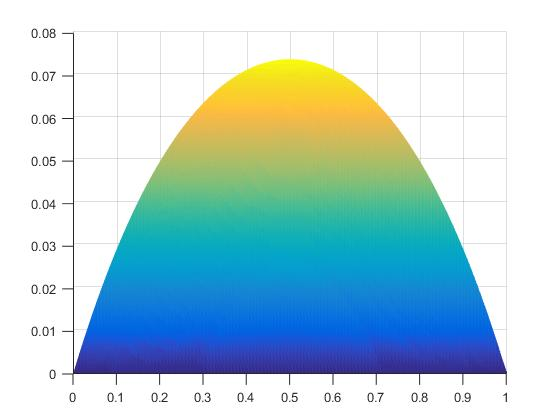
\includegraphics[scale=0.3]{solution2.jpg}
	\end{frame}	
	
		\begin{frame}{Fall 1: 1 0 2}
\begin{center}
	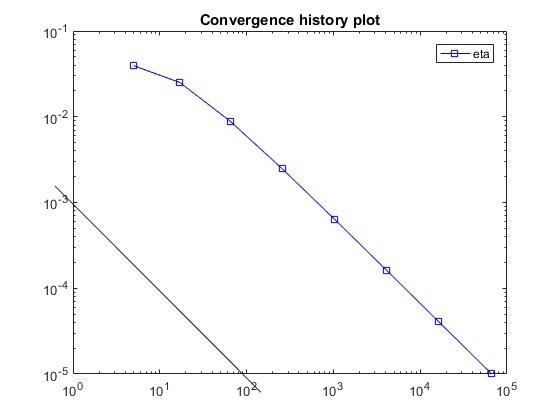
\includegraphics[scale=0.3]{102.jpg}
\end{center}

	\end{frame}	
	
			\begin{frame}{Fall 1: 2 1 3}
\begin{center}
	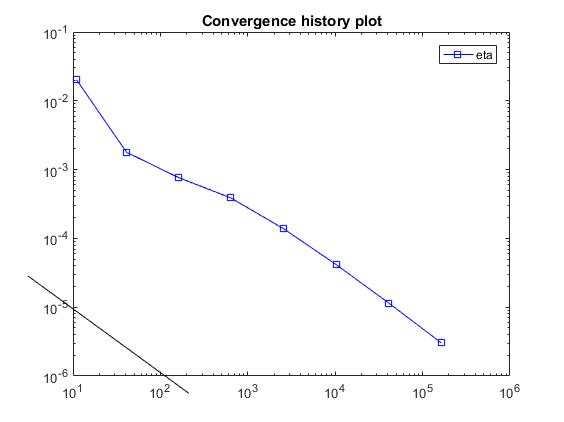
\includegraphics[scale=0.3]{213.jpg}
\end{center}

	\end{frame}	
	
				\begin{frame}{Fall 2: 1 1 2 }
\begin{center}
	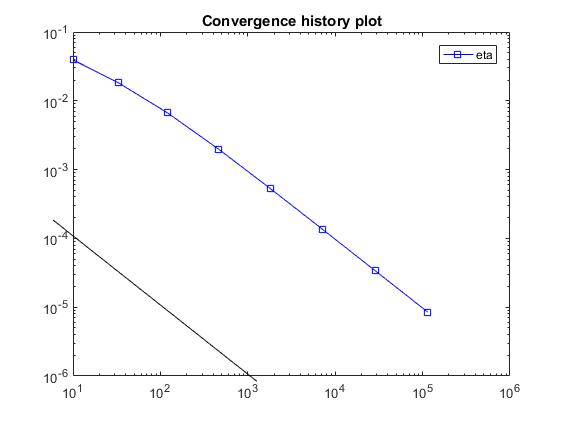
\includegraphics[scale=0.3]{112.jpg}
\end{center}

	\end{frame}	
	
				\begin{frame}{Fall 2: 2 2 3}
\begin{center}
	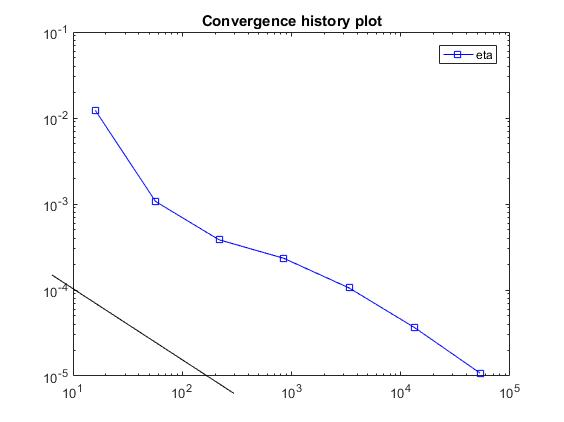
\includegraphics[scale=0.3]{223.jpg}
\end{center}
	\end{frame}	

				\begin{frame}{Fall 3: 1 0 1}
\begin{center}
	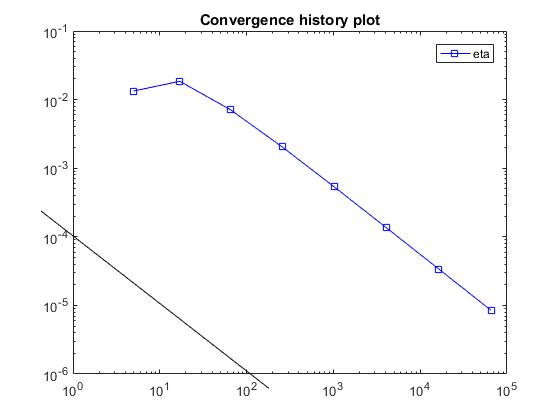
\includegraphics[scale=0.3]{101.jpg}
\end{center}
	\end{frame}	
					\begin{frame}{Fall 3: 2 1 2}
\begin{center}
	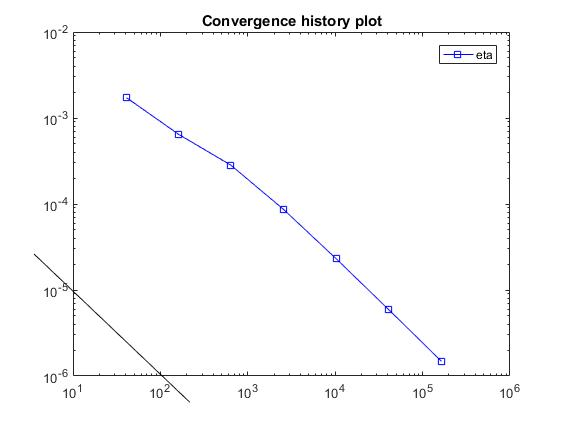
\includegraphics[scale=0.3]{212.jpg}
\end{center}
	\end{frame}	

				\begin{frame}{Fall 3: 3 2 3}
\begin{center}
	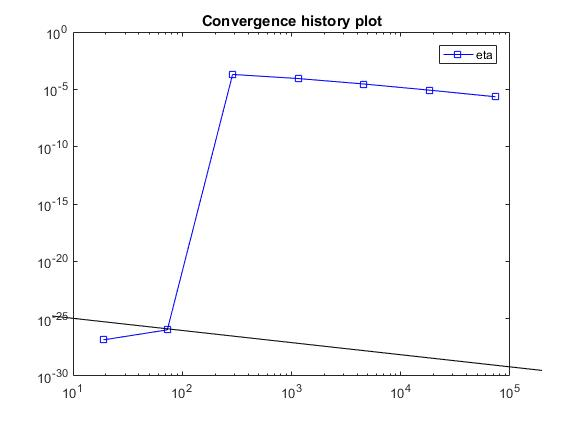
\includegraphics[scale=0.3]{323.jpg}
\end{center}
	\end{frame}	

				\begin{frame}{Vergleich 1 0 1 und 3 2 3 - ,,Höhenuntererschied''}
\begin{center}
	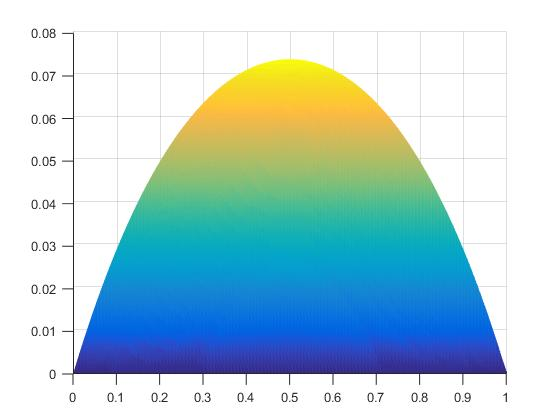
\includegraphics[scale=0.3]{solution2.jpg}
	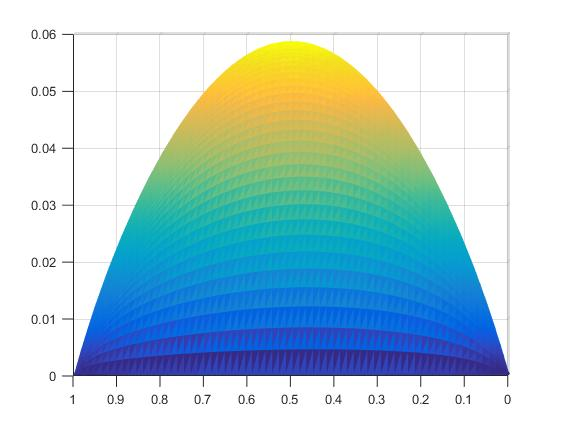
\includegraphics[scale=0.3]{figureweird.jpg}
\end{center}
	\end{frame}	
	
\begin{frame}{Problem aus dem Paper}
\begin{center}
Die Funktion $f$ für das Poisson-Problem \\
$-\Delta u =f$ \\
wird so gewählt, dass die exakte Lösung\\
 $u=\sin (\pi x) \sin (\pi y)$ 
 ist, \\
 also gilt 
 $f=2\pi ^2 \sin (\pi x) \sin (\pi y)$ und  $u_{|\partial \Omega}=0  $
\end{center}
\end{frame}	


	
	
					\begin{frame}{Vergleich 1 0 1 und 3 2 3 für $f=2\pi ^2 \sin (\pi x) \sin (\pi y)$}
\begin{center}
	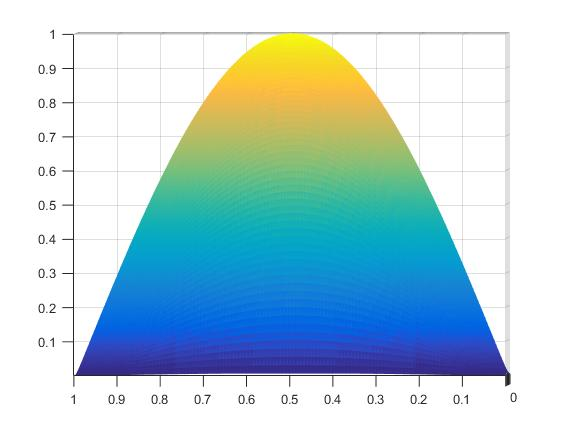
\includegraphics[scale=0.25]{101p.jpg}
	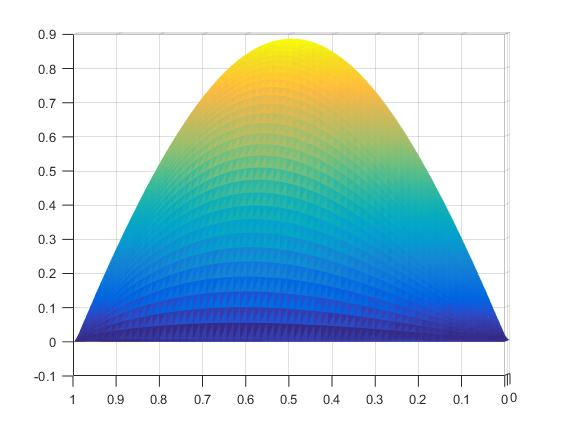
\includegraphics[scale=0.25]{323p.jpg}\\
	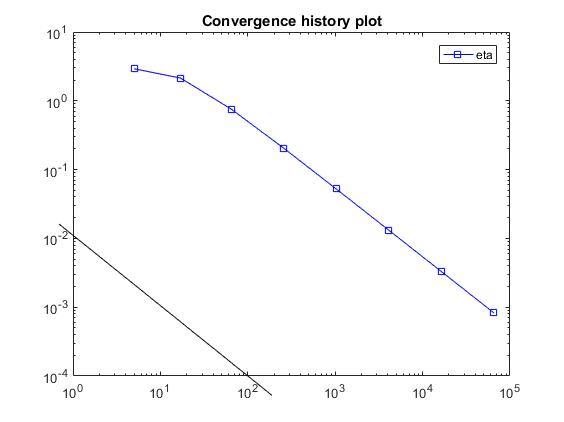
\includegraphics[scale=0.25]{101plot.jpg}
	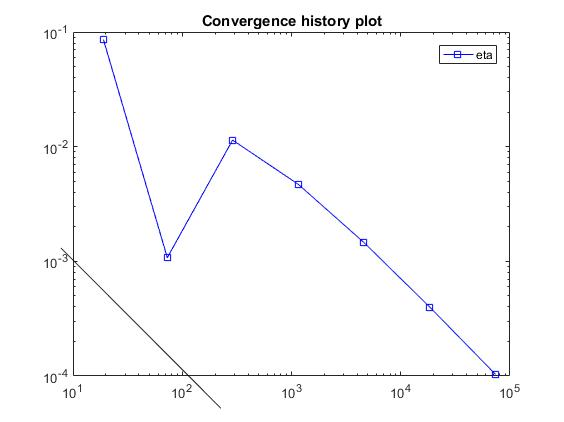
\includegraphics[scale=0.25]{323plot.jpg}
\end{center}

\end{frame}	

				\begin{frame}{Triangulierung kein- und einmal rotverfeinert.}
\begin{center}
	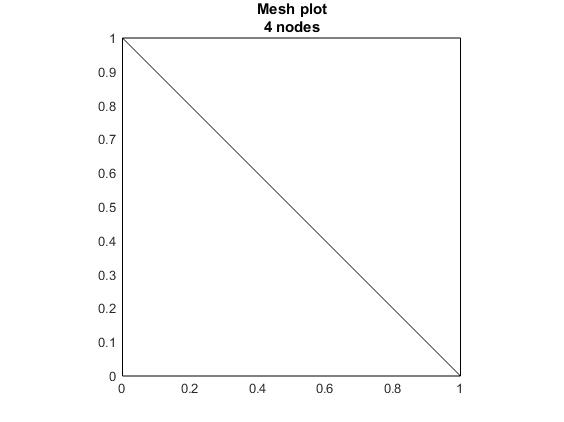
\includegraphics[scale=0.3]{tri0.jpg}
	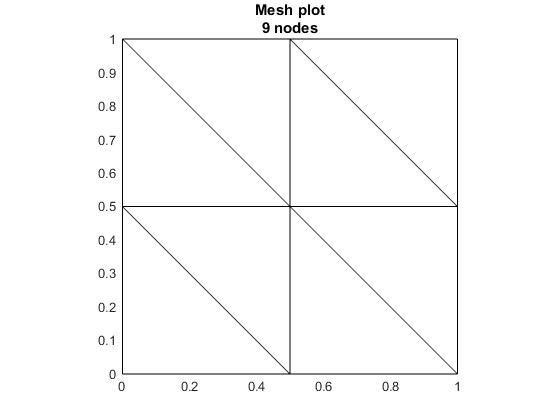
\includegraphics[scale=0.3]{tri1.jpg}
\end{center}
	\end{frame}	

\begin{frame}{$H_1$-Konvergenzrate}

$$ \mathrm{log}_2\left( \frac{\left\Vert u-u_h  \right\Vert_{\Hh^1(\Omega)}  }{ \left\Vert u-u_{h/2}  \right\Vert_{\Hh^1(\Omega)}}   \right)$$
\end{frame}

\begin{frame}{Checkliste}
\begin{itemize}
  \item
  \begin{todolist}
  \item[\done] $P_1$ implementieren.
  \item[\done] $P_2$ implementieren.
\pause  
  \item[\done] $P_3$ implementieren.
  \item[\done] Implementation des eingebauten Fehlerschätzers.
  \pause
  \item Nachstellen der Experimente aus dem Paper.
  \pause
  \item[\wontfix] Optimierung des Codes.
  \item[\wontfix] Durchführung weiterer Experimente.
  \item[\wontfix] Auswertung und Dokumentation.
  
  \end{todolist}
\end{itemize}
\end{frame}		

	
\end{document}